%  encoding : utf8 
%  TKZdoc-aq.tex
%  Created by Alain Matthes  on 2009-03-13.
%  Copyright (C) 2009 Alain Matthes  
%
% This file may be distributed and/or modified
%
% 1. under the LaTeX Project Public License , either version 1.3
% of this license or (at your option) any later version and/or
% 2. under the GNU Public License.
% See http://www.latex-project.org/lppl.txt for details.
%
%
% 'doc-aq' is the french doc of alterqcm.sty
%
%
%%%%%%%%%%%%%%%%%%%%%%%%%%%%%%%%%%%%%%%%%%%%%%%%%%%%%%%%%%%%%%%%%
%                                                               %
%   doc   altermqcm.sty    encodage : utf8                      %
%                                                               %
%%%%%%%%%%%%%%%%%%%%%%%%%%%%%%%%%%%%%%%%%%%%%%%%%%%%%%%%%%%%%%%%%
%                                                               %
%           Créé par Alain Matthes le 20/04/2009                %
%  Copyright (c) 2009 __Collège Sévigné__ All rights reserved.  %
%        version : 3.7                                          %
%%%%%%%%%%%%%%%%%%%%%%%%%%%%%%%%%%%%%%%%%%%%%%%%%%%%%%%%%%%%%%%%%

% Fichier  .tex de présentation du package alterqcm.sty
% d'après le code de DTK.
\documentclass[DIV=15,
               fontsize=10,
               headinclude=false,
               index=totoc,
               footinclude=false,
               twoside,
               headings=small]{tkz-doc}

\usepackage{fancybox}
\usepackage{stmaryrd}
\usepackage{array,multirow,longtable,tkz-tab,tkz-base}
\usepackage{alterqcm} 

\usepackage[pdftex,unicode,
                colorlinks=true,
                pdfpagelabels, 
                urlcolor=blue,
                filecolor=pdffilecolor,
                linkcolor=blue,
                breaklinks =false,
                hyperfootnotes=false,
                bookmarks=false,
                bookmarksopen=false, 
                linktocpage=true,
                pdfsubject={qcm},
                pdfauthor={Alain Matthes},
                pdftitle={alterqcm},
                pdfkeywords={qcm, mathematics, table},
                pdfcreator={LaTeX}
                ]{hyperref}  
\usepackage{url}
\def\UrlFont{\small\ttfamily}
\usepackage[protrusion = true,
            expansion,
            final,
            verbose = false,
            babel   = true]{microtype} 

\DisableLigatures{encoding = T1, family = tt*}   
\usepackage[parfill]{parskip}

\gdef\nameofpack{alterqcm}
\gdef\versionofpack{3.7 c}
\gdef\dateofpack{2011/06/01}
\gdef\nameofdoc{doc-alterqcm}
\gdef\versionofdoc{3.7 c}   
\gdef\dateofdoc{2011/06/01}
\gdef\authorofpack{Alain Matthes}
\gdef\adressofauthor{}
\gdef\namecollection{AlterMundus}
\gdef\urlauthor{http://altermundus.fr}
\gdef\urlauthorcom{http://altermundus.com} 
   
\title{The package : alterqcm.sty}
\author{Alain Matthes}
\pdfcompresslevel=9
\pdfinfo{
    /Title (doc_alterqcm.pdf)
    /Creator (TeX)
    /Producer (pdfeTeX)
    /Author (Alain Matthes)
    /CreationDate (01 juin 2011)
    /Subject (Documentation du package alterqcm v 3.7)
    /Keywords (pdfeTeX, qcm, maths, pdflatex) }  



\renewcommand*{\Ienv}[1]{\index{Environnement_1@\texttt{Environnement}!\texttt{#1}}}
\renewcommand*{\NameSys}[1]{\index{Système d'exploitation !#1@\texttt{#1}}}

\usepackage{shortvrb,verbdef,fancyvrb} 
\usepackage{tkzexample} 
\usepackage[frenchb]{babel}
\usepackage[autolanguage]{numprint}  
 
\makeatletter
\renewcommand*\l@subsubsection{\bprot@dottedtocline{3}{3.8em}{4em}}  
\makeatother
\AtBeginDocument{\MakeShortVerb{\|}}

\begin{document}
%<–––––––––––––––––––––––––––––––––––––––––––––––––––––––––––––––––––––––––––>   
\title{\nameofpack}
\date{\today}
\clearpage
\thispagestyle{empty}
\maketitle
\clearpage 
\definecolor{fondpaille}{cmyk}{0,0,0.1,0}
\colorlet{graphicbackground}{fondpaille}
\colorlet{codebackground}{brown!15}
\colorlet{codeonlybackground}{brown!15} 
\pagecolor{fondpaille}
\color{Maroon} 

\nameoffile{\nameofpack} 
\defoffile{\textbf{alterqcm.sty} est un package pour mettre en page le plus simplement possible des questionnaires à choix multiples sous forme de tableaux à deux colonnes.}

\presentation

\vspace*{12pt}

\lefthand\ Je remercie  \tkzimp{Michel Bovani} pour nous permettre d'utiliser \tkzname{fourier} et \tkzname{utopia} avec \LaTeX.

\vspace*{12pt}
\lefthand\ Je remercie également  \tkzimp{Jean-Côme Charpentier},  \tkzimp{Manuel Pégourié-Gonnard},  \tkzimp{Franck Pastor}, \tkzimp{Ulrike Fischer} et \tkzimp{Josselin Noirel}  pour les différentes idées et conseils qui m'ont permis de faire ce package.

\vfill
Vous pouvez envoyer vos remarques, et les rapports sur des erreurs que vous aurez constatées
 à l'adresse suivante  \href{mailto:al.ma@mac.com}{\textcolor{blue}{Alain Matthes}}
 
 
This file can be redistributed and/or modified under the terms of the LATEX 
Project Public License Distributed from CTAN archives in directory \url{CTAN:// 
macros/latex/base/lppl.txt}. 

\clearpage\newpage
\setlength{\parskip}{1ex plus 0.5ex minus 0.2ex}  

\tableofcontents
%<–––––––––––––––––––––––––––––––––––––––––––––––––––––––––––––––––––––––––––> 
%!TEX root = /Users/ego/Boulot/Alterqcm/doc/doc_aq-main.tex   

\section{Installation.}

\subsection{Avec TeXlive sous Linux ou OS X}\NameDist{TeXLive}\NameSys{Linux}
\NameDist{MacTeX}\NameSys{OS X}
\tkzname{alterqcm}  est présent sur les serveurs du \tkzname{CTAN} et fait   partie de \tkzname{TeXLive} alors  \tkzname{tlmgr} vous permettra de l'installer.  Si  \tkzname{alterqcm} ne fait pas encore partie de votre distribution, cette section vous montre comment l'installer, elle est aussi nécessaire si vous avez envie d'installer une version beta  ou personnalisée de \tkzname{alterqcm}. 

Le plus simple est de créer un dossier \tikz[remember picture,baseline=(n1.base)]\node [fill=blue!30,draw] (n1) {prof};\footnote{ou bien un autre nom}  avec comme chemin : \colorbox{blue!20}{ texmf/tex/latex/prof}. Voici les chemins de ce dossier sur mes deux ordinateurs:

\medskip
\begin{itemize}\setlength{\itemsep}{5pt}

\item   sous OS X \colorbox{blue!30}{\textbf{/Users/ego/Library/texmf}}; 

\item   sous Ubuntu \colorbox{blue!30}{\textbf{/home/ego/texmf}}.
\end{itemize}

Je suppose que si vous mettez vos packages ailleurs, vous savez pourquoi !

L'installation que je propose n'est valable que pour un utilisateur. 

\medskip
\begin{enumerate}
\item Téléchargez le fichier \tikz[remember picture,baseline=(n2.base)]\node [fill=blue!20,draw] (n2) {alterqcm.sty}; sur l'un des serveurs  du \tkzname{CTAN}.

\item Placez le fichier \tikz[remember picture,baseline=(n2.base)]\node [fill=blue!20,draw] (n2) {alterqcm.sty}; dans le dossier \tkzname{latex}  ou bien  dans un dossier personnel \tikz[baseline=(tk.base)]\node [fill=blue!30,draw] (tk) {prof};.
\begin{itemize}\setlength{\itemsep}{5pt}

\item  \colorbox{blue!30}{\textbf{\texttildelow/Library/texmf/latex}}; 

\item   \colorbox{blue!30}{\textbf{\texttildelow/Library/texmf/latex/prof}}.
\end{itemize}   


\item Ouvrir un terminal, puis faire \colorbox{red!20}{|sudo texhash|} si nécessaire.

\end{enumerate} 


\subsection{Avec MikTeX sous Windows XP}\NameDist{MikTeX}\NameSys{Windows XP}


Je ne connais pas grand-chose à ce système, mais un utilisateur de mes packages \tkzimp{Wolfgang Buechel} a eu la gentillesse de me faire parvenir ce qui suit~:

Pour ajouter \tkzname{alterqcm.sty} à MiKTeX\footnote{Essai réalisé avec la version \tkzname{2.7}}:

\begin{itemize}\setlength{\itemsep}{10pt}
  \item ajouter un dossier \tkzname{prof} dans le dossier
       \textcolor{blue!60!black}{\texttt{[MiKTeX-dir]/tex/latex}}
  \item copier  le fichier  \tkzname{alterqcm.sty} dans le dossier \tkzname{prof},
  \item mettre à jour  MiKTeX, pour cela dans shell DOS lancer la commande   \textbf{\textcolor{red}{|mktexlsr -u|}} 
  
   ou bien encore, choisir \textcolor{red!50}{|Start/Programs/Miktex/Settings/General|}
   
    puis appuyer sur le bouton  \textbf{\textcolor{red}{|Refresh FNDB|}}.
\end{itemize}      

\endinput


%!TEX root = /Users/ego/Boulot/Alterqcm/doc/doc_aq-main.tex     
\section{Les outils : L' environnement \tkzname{alterqcm} et la macro  \tkzcname{AQquestion}}
\subsection{L' environnement \tkzname{alterqcm}}


\bigskip
\begin{NewEnvBox}{alterqcm} 

\noindent Voici la liste des \tkzname{options} disponibles classées par catégories.

\medskip
\begin{tabular}{@{}Il Il Il@{}} 
	\toprule
	\thead
Options                &Défaut          & Définition                                \\ \midrule
\tbody
\multicolumn{2}{c}{\emph{\texttt{Dimensions}}} \\ \cmidrule(r){1-2}
\TOenvline{lq}        {100mm}  {largeur de la colonne question            }
\TOenvline{pq}        {0pt}    {déplacement vertical de la question       } \cmidrule(r){1-2}
\multicolumn{2}{c}{\emph{\texttt{Nombres}}} \\ \cmidrule(r){1-2}
\TOenvline{bonus}     {{0,5}}  {points attribués à une bonne réponse      }
\TOenvline{malus}     {{0,25}} {points attribués à une mauvaise réponse   }
\TOenvline{numbreak}  {0}    {pour reprendre un tableau scindé          }
\TOenvline{points}  {empty}{ points attribués au qcm dans la marge} \cmidrule(r){1-2}
\multicolumn{2}{c}{\emph{\texttt{Macros}}} \\ \cmidrule(r){1-2}
\TOenvline{symb}      {\$\BS square\$} {symbole devant la proposition     }
\TOenvline{corsymb}{\$\BS blacksquare\$}{symbole devant la proposition    }
\TOenvline{numstyle}  {\BS arabic} {style de la numérotation des questions  }
\TOenvline{propstyle} {\BS alph} {style de la numérotation des propositions }
\TOenvline{size}  {\BS normalsize} {taille de la fonte           }
\TOenvline{afterpreskip}{\BS medskip} {skip après la présentation  }  
\cmidrule(r){1-2}
\multicolumn{2}{c}{\emph{\texttt{Booléens}}} \\ \cmidrule(r){1-2}
\TOenvline{long}      {true}     {longtable à la place de tabular   }
\TOenvline{sep}       {true}  {filet de séparation entre les propositions}
\TOenvline{pre}       {false}  {présentation du QCM          }
\TOenvline{VF}        {false}  {QCM sous la forme Vrai ou Faux }
\TOenvline{numprop}   {false}  {numérotation des propositions    }
\TOenvline{num}       {true}   {style de la numérotation des questions  }
\TOenvline{nosquare}  {false}   {suppression du carré des propositions     }
\TOenvline{title}     {false} {suppression des titres                    }
\TOenvline{correction}{false} {permet de créer un corrigé                }
\TOenvline{alea}      {false}  {placer des propositions aléatoirement     } \cmidrule(r){1-2}
\multicolumn{2}{c}{\emph{\texttt{Textes}}} \\ \cmidrule(r){1-2}
\TOenvline{tone}     {Questions} {titre colonne 1                           }
\TOenvline{ttwo}     {R\'eponses} {titre colonne 2     } 
\TOenvline{language}  {french}  {french, english ou german   }
 \bottomrule
\end{tabular}

\medskip

\emph{Il suffit donc pour créer un \textcolor{red}{\texttt{QCM}} d'utiliser un environnement \textcolor{red}{\texttt{alterqcm}} ainsi que la macro \textcolor{red}{ \addbs{AQquestion}} définie dans la section suivante.}
\end{NewEnvBox} 

\newpage
\subsection{La commande \tkzcname{AQquestion}} 
\Imacro{AQquestion}

\begin{NewMacroBox}{AQquestion}{\oarg{local options}{\var{quest}}\{{\var{$\mathrm{prop}_1$}},\ldots,{\var{$\mathrm{prop}_n$}}\}}
Cette macro utilise deux arguments, le premier définit la question, le second est une liste qui définit les propositions.

\medskip
\begin{tabular}{@{}Il Il Il@{}}  \toprule \thead
arguments                 & défaut           & définition    \\ 
\midrule
\tbody
\TAline{quest}  {}     {définition de la question}          
\TAline{$\mathrm{prop}_i$}  {}     {i\ieme\ proposition}       \bottomrule
\end{tabular}

\medskip
Voici la liste des options liées à cette macro.

\medskip
\begin{tabular}{@{}Il Il Il@{}}  \toprule \thead
options                 & défaut           & définition                    \\ \midrule
\tbody
\TOline{pq}  {0pt}     {ajustement de la position de la question}   
\TOline{br}  {1  }     {liste de rangs des bonnes réponses  }           \bottomrule
\end{tabular}
  
\medskip

\end{NewMacroBox}
 
\subsection{Utilisation : premier exemple}

Il suffit d'utiliser un environnement \tkzname{alterqcm} et la macro \tkzcname{AQquestion}, voici un exemple :


 \noindent
\begin{minipage}[c][][t]{.40\linewidth}  
\begin{tkzexample}[code only,small]
 \documentclass[12pt]{article}
 \usepackage[utf8]{inputenc}
 \usepackage[upright]{fourier}
 %\usepackage[T1]{fontenc}
 %\usepackage{lmodern}
 \usepackage{alterqcm}
 \usepackage{fullpage}
 %\usepackage{longtable} 
 % nécessaire pour l'option "long"
 \usepackage[frenchb]{babel}
 \parindent0pt
 \begin{document}
 \begin{alterqcm} 
  \AQquestion{Question}{% 
  {Proposition 1},
  {Proposition 2},
  {Proposition 3}}
 \end{alterqcm}
 \end{document}\end{tkzexample}
\end{minipage}\hfill \noindent  
\begin{minipage}[c][][b]{.50\linewidth}
\textbf{alterqcm.sty} crée un nouvel environnement \textbf{alterqcm} qui permet l'obtention d'un tableau à deux colonnes. La colonne de gauche pour les questions, l'autre pour les différentes propositions.  Les propositions sont données dans une liste :

\tkzname{\{\{Proposition 1\},\\\{Proposition 2\},\\\{Proposition 3\}\}}.

 Le nombre de propositions est compris entre \tkzname{2} et \tkzname{5}.
\end{minipage}

\medskip
Ce qui donne comme résultat :

\bigskip
  \begin{alterqcm}
  \AQquestion{Question}
  {%
  {Proposition 1},
  {Proposition 2},
  {Proposition 3}%
  }
  \end{alterqcm}

\medskip
 La largeur totale du tableau est égale à \tkzcname{textwidth}. Par défaut la  colonne question a pour largeur \tkzname{100mm} plus quelques millimètres ... introduits par le tableau. La largeur des réponses est égale à \tkzcname{textwidth} diminuée de la largeur de la première colonne. \Imacro{textwidth}

Le point important est que la hauteur des lignes des propositions soit calculée automatiquement afin, d'une part, que le texte des propositions soit placé correctement sans toucher les filets et d'autre part, que le texte de la question correspondante puisse être inclus dans sa case. Un positionnement précis est obtenu avec l'option \tkzname{pq}.  

\subsection{Packages chargés par \tkzname{alterqcm.sty}}
La liste des packages chargés est la suivante :

\begin{tkzexample}[code only]
	\RequirePackage{xkeyval}[2005/11/25]
	\RequirePackage{calc}
	\RequirePackage{ifthen,forloop}
	\RequirePackage{array}
	\RequirePackage{multirow}
	\RequirePackage{pifont}
\end{tkzexample}
\NamePack{xkeyval}\NamePack{calc}\NamePack{ifthen}\NamePack{forloop}\NamePack{array}\NamePack{multirow}
\NamePack{pifont}

Il vous sera nécessaire de charger \tkzname{longtable.sty} si vous souhaitez utiliser l'option \tkzname{long} pour un de vos tableaux. Vous avez besoin aussi de la macro \tkzcname{square}, elle est soit définie dans le package \tkzname{fourier}, soit dans le package \tkzname{amsmath}.\NamePack{amsmath}\NamePack{fourier}.


 \subsection{Utilisation de l'environnement \tkzname{minipage} pour modifier la largeur du tableau}
\Ienv{minipage}

\begin{minipage}[c][][t]{.3\linewidth}
\begin{tkzltxexample}[small]

 \begin{center}
 \begin{minipage}{9cm}
  \begin{alterqcm}[lq=5cm]
    ...
  \end{alterqcm}
 \end{minipage}
 \end{center}
\end{tkzltxexample}
\end{minipage}\hfill 
\begin{minipage}[c][][t]{.6\linewidth}
\begin{alterqcm}[lq=5cm]
\AQquestion{Parmi les propositions suivantes, quelle est celle qui permet%
 d'affirmer que la fonction exponentielle  admet pour asymptote la droite%
  d'équation $y = 0$ ?}
{%
{$\displaystyle\lim_{x \to +\infty} \text{e}^x = + \infty$},%
{$\displaystyle\lim_{x \to -\infty} \text{e}^x = 0$},%
{$\displaystyle\lim_{x \to +\infty} \dfrac{\text{e}^x}{x} = + \infty$}%
}

\AQquestion[]{exp$(\ln x) = x$ pour tout $x$ appartenant à }
{%
{$\mathbf{R}$},%
{$\big]0~;~+ \infty\big[$},%
{$\big[0~;~+\infty\big[$}%
}\end{alterqcm}
\end{minipage} 
% 


\subsection{Modification temporaire de \tkzcname{textwidth}}
\Imacro{textwidth}
 Il est possible d'utiliser des tableaux ainsi que d'autres structures dans le code de la question ou encore des propositions. Voici un exemple :
\newlength{\oldtextwidth}

\begin{tkzltxexample}[small]
	\newlength{\oldtextwidth}
\end{tkzltxexample}

\medskip
	\setlength{\oldtextwidth}{\textwidth}
	\setlength{\textwidth}{14cm}
\begin{alterqcm}[lq=88mm,symb=$\Box$]
 \AQquestion{la matrice%
 \( M=\begin{pmatrix}
        0 & 1 \\
        1 & 1 \\
\end{pmatrix} \)  a pour carré}%
{%
{\(\begin{pmatrix}
        0 & 1 \\
        1 & 4 \\
\end{pmatrix}\)},%
{\(\begin{pmatrix}
        1 & 2 \\
        2 & 5 \\
 \end{pmatrix}\)}
}
\end{alterqcm}
\setlength{\textwidth}{\oldtextwidth}  

\medskip
\begin{tkzltxexample}[small]
  \setlength{\oldtextwidth}{\textwidth}
  \setlength{\textwidth}{14cm}
 \begin{alterqcm}[lq=88mm,symb=$\Box$]
  \AQquestion{la matrice%
  \( M=\begin{pmatrix}
         0 & 1 \\
         1 & 1 \\
 \end{pmatrix} \)  a pour carré}%
 {%
 {\(\begin{pmatrix}
         0 & 1 \\
         1 & 4 \\
 \end{pmatrix}\)},%
 {\(\begin{pmatrix}
         1 & 2 \\
         2 & 5 \\
  \end{pmatrix}\)}
 }
 \end{alterqcm}
 \setlength{\textwidth}{\oldtextwidth}
\end{tkzltxexample}



\endinput
%!TEX root = /Users/ego/Boulot/Alterqcm/doc/doc_aq-main.tex
\section{Options globales de l'environnement  \tkzname{alterqcm}}

\subsection{\tkzname{lq} : modification de la largeur de la première colonne }
\IoptEnv{alterqcm}{lq}

\begin{alterqcm}[long,lq=110mm]
\AQquestion{Parmi les propositions suivantes, quelle est celle qui permet %
 d'affirmer que la fonction exponentielle  admet pour asymptote %
  la droite d'équation $y = 0$ ?}
{{$\displaystyle\lim_{x \to +\infty} \text{e}^x = + \infty$},
{$\displaystyle\lim_{x \to -\infty} \text{e}^x = 0$},
{$\displaystyle\lim_{x \to +\infty} \dfrac{\text{e}^x}{x} = + \infty$}}

\AQquestion{exp$(\ln x) = x$ pour tout $x$ appartenant à }
{{$\mathbb{R}$},
{$\big]0~;~+ \infty\big[$},
{$\big[0~;~+\infty\big[$}
}
\end{alterqcm}

\medskip
Voyons le code nécessaire pour obtenir ce tableau. Il faut  placer
\tkzcname{usepackage\{alterqcm\}} dans le préambule. Il faut remarquer que seule la largeur de la colonne des questions est fournie |lq=100mm| et que cela est optionnel. Le nombre des propositions est ici \textbf{3} mais il peut varier d'une question à l'autre.

\begin{tkzexample}[code only,small]
 \begin{alterqcm}[long,lq=110mm]
  \AQquestion{Parmi les propositions suivantes, quelle est celle qui permet %
  d'affirmer que la fonction exponentielle  admet pour asymptote %
    la droite d'équation $y = 0$ ?}
  {{$\displaystyle\lim_{x \to +\infty} \text{e}^x = + \infty$},
  {$\displaystyle\lim_{x \to -\infty} \text{e}^x = 0$},
  {$\displaystyle\lim_{x \to +\infty} \dfrac{\text{e}^x}{x} = + \infty$}}
  
  \AQquestion[]{exp$(\ln x) = x$ pour tout $x$ appartenant à }
  {{$\mathbb{R}$},
  {$\big]0~;~+ \infty\big[$},
  {$\big[0~;~+\infty\big[$}
  }
  \end{alterqcm}\end{tkzexample}



\subsection{\tkzname{pq} : utilisation globale }
 \IoptEnv{alterqcm}{pq}  

Cette fois, il est nécessaire de déplacer plusieurs questions, j'ai placé un |pq=2mm| globalement c'est à dire comme ceci :\tkzcname{begin\{alterqcm\}[lq=85mm,pq=2mm]}. \textbf{Toutes} les questions sont affectées par cette option mais certaines questions  étaient bien placées et doivent le rester, aussi localement je leur redonne un |pq=0mm|.

\medskip
\begin{alterqcm}[lq=85mm,pq=2mm]
\AQquestion{Soit une série statistique à deux variables. Les valeurs de $x$ sont 1, 2, 5, 7, 11, 13 et une équation de la droite de régression de $y$ en $x$ par la moindres carrés est $y = 1,35x +22,8$. Les coordonnées du point moyen sont :}
{{$(6,5;30,575)$},
{$(32,575 ; 6,5)$},
{$(6,5 ; 31,575)$}}

\AQquestion{Pour tout réel $x$, le nombre \[\dfrac{\text{e}^x - 1}{\text{e}^x + 2}\hskip12pt \text{égal à :} \] }
{{$-\dfrac{1}{2}$},
{$\dfrac{\text{e}^{-x} - 1}{\text{e}^{-x} + 2}$},
{$\dfrac{1 - \text{e}^{-x}}{1 + 2\text{e}^{-x}}$}
}
\AQquestion{On pose I $= \displaystyle\int_{\ln 2}^{\ln 3} \dfrac{1}{\text{e}^x - 1}\,\text{d}x$ et J $ = \displaystyle\int_{\ln 2}^{\ln 3} \dfrac{\text{e}^x}{\text{e}^x - 1}\,\text{d}x$ \\ alors le nombre  I $-$ J est égal à}
{{$\ln \dfrac{2}{3}$},
{$\ln \dfrac{3}{2}$},
{$\dfrac{3}{2}$}
}
\end{alterqcm}

\begin{tkzexample}[code only,small]
 \begin{alterqcm}[lq=85mm,pq=2mm]
 \AQquestion{Pour tout réel $x$, le nombre \[\dfrac{\text{e}^x - 1}
 {\text{e}^x + 2}\hskip12pt \text{égal à :} \] }
 {{$-\dfrac{1}{2}$},
 {$\dfrac{\text{e}^{-x} - 1}{\text{e}^{-x} + 2}$},
 {$\dfrac{1 - \text{e}^{-x}}{1 + 2\text{e}^{-x}}$}}
 \end{alterqcm}
\end{tkzexample}


\subsection{\tkzname{VF} : Vrai ou Faux}
\IoptEnv{alterqcm}{VF}
Les propositions ne sont que  deux et le candidat doit choisir entre \textbf{Vrai} ou \textbf{Faux}. Cette fois, la syntaxe est allégée. Il n'est plus nécessaire d'écrire la liste des propositions et  il suffit de positionner \tkzname{VF}  en plaçant dans les options   \tkzname{$VF$}.

 
\begin{minipage}[t][][b]{.45\linewidth}
Soit $f$ une fonction définie et dérivable sur l'intervalle $\big[-3~;~+\infty\big[$, croissante sur les intervalles $\big[-3~;~-1\big]$ et $\big[2~;~+\infty\big[$ et décroissante sur l'intervalle $\big[-1~;~2\big]$.

 On note $f'$ sa fonction dérivée sur l'intervalle $[-3~;~+\infty[$.

La courbe $\Gamma$ représentative de la fonction $f$ est tracée ci-dessous dans un repère orthogonal $\big(O,~\vec{\imath},~\vec{\jmath}\big)$.

Elle passe par le point A$(-3~;~0)$ et admet pour asymptote la droite $\Delta$ d'équation $y =  2x -5$.
\end{minipage}
\hfill
\begin{minipage}[t][][b]{.45\linewidth}
\null
\begin{tikzpicture}[scale=0.5,>=latex]
 \draw[very thin,color=gray] (-3,-2) grid (10,8);
 \draw[->] (-3,0) -- (10,0) node[above left] {\small $x$};
 \foreach \x in {-3,-2,-1,1,2,...,9}
    \draw[shift={(\x,0)}] (0pt,1pt) -- (0pt,-1pt)node[below] { $\x$};
 \draw[->] (0,-2) -- (0,8) node[below right] {\small $y$};
 \foreach \y/\ytext in {-2,-1,1,2,...,7}
    \draw[shift={(0,\y)}] (1pt,0pt) -- (-1pt,0pt) node[left] { $\y$};
 \draw (2,-1) -- (6,7);
 \node[above right] at (-3,0) {\textbf{A}};
 \node[above right] at (0,0) {\textbf{O}};
 \node[below right] at (4,3) {$\mathbf{\Delta}$};
 \node[above right] at (4,5) {$\mathbf{\Gamma}$};
 \draw plot[smooth] coordinates{%
 (-3,0)(-2,4.5)(-1,6.5)(0,5.5)(1,3.5)(2,3)(3,3.4)(4,4.5)(5,6)(6,7.75)};
\end{tikzpicture}
\end{minipage}
                     

\begin{alterqcm}[VF,lq=125mm]
 \AQquestion{Pour tout $x \in ]-3~;~2],~f'(x) \geqslant 0$.}
 \AQquestion{La fonction $F$ présente un maximum en $2$}
 \AQquestion{$\displaystyle\int_{0}^2 f'(x)\,\text{d}x = - 2$}
\end{alterqcm}

\begin{tkzexample}[code only, small]
 \begin{minipage}[t][][b]{.45\linewidth}
  Soit $f$ une fonction définie et dérivable sur l'intervalle $\big[-3~;~+\infty\big[$,
   croissante sur les intervalles $\big[-3~;~-1\big]$ et $\big[2~;~+\infty\big[$
   et décroissante sur l'intervalle $\big[-1~;~2\big]$.
  
   On note $f'$ sa fonction dérivée sur l'intervalle $[-3~;~+\infty[$.
  
  La courbe $\Gamma$ représentative de la fonction $f$ est tracée ci-dessous
   dans un repère orthogonal $\big(O,~\vec{\imath},~\vec{\jmath}\big)$.
  
  Elle passe par le point A$(-3~;~0)$ et admet pour asymptote la droite
  $\Delta$ d'équation $y =  2x -5$.
 \end{minipage}
 \begin{minipage}[t][][b]{.45\linewidth}
 \null
\begin{tikzpicture}[scale=0.5,>=latex]
  \draw[very thin,color=gray] (-3,-2) grid (10,8);
  \draw[->] (-3,0) -- (10,0) node[above left] {\small $x$};
  \foreach \x in {-3,-2,-1,1,2,...,9}
     \draw[shift={(\x,0)}] (0pt,1pt) -- (0pt,-1pt)node[below] { $\x$};
  \draw[->] (0,-2) -- (0,8) node[below right] {\small $y$};
  \foreach \y/\ytext in {-2,-1,1,2,...,8}
     \draw[shift={(0,\y)}] (1pt,0pt) -- (-1pt,0pt) node[left] { $\y$};
  \draw (-0.5,-2) -- (10,8);
  \node[above right] at (-3,0) {\textbf{A}};
  \node[above right] at (0,0) {\textbf{O}};
  \node[below right] at (4,3) {$\mathbf{\Delta}$};
  \node[above right] at (4,5) {$\mathbf{\Gamma}$};
  \draw plot[smooth] coordinates{%
  (-3,0)(-2,4.5)(-1,6.5)(0,5.5)(1,3.5)(2,3)(3,3.4)(4,4.5)(5,6)(6,7.75)};
 \end{tikzpicture}
 \end{minipage}
 \begin{alterqcm}[VF,lq=125mm]
   \AQquestion{Pour tout $x \in ]-\infty~;~2],~f'(x) \geqslant 0$.}
   \AQquestion{La fonction $F$ présente un maximum en $2$}
   \AQquestion{$\displaystyle\int_{0}^2 f'(x)\:\text{d}x = - 2$}
 \end{alterqcm}
\end{tkzexample}

\subsection{\tkzname{symb} : modification du symbole } 
\IoptEnv{alterqcm}{symb}

 Si vos fontes ne possèdent pas le symbole |$\square$| ou encore |$\blacksquare$| vous pouvez utiliser celui fourni par le package ou bien en créer un vous même. \tkzcname{altersquare}, \tkzcname{dingsquare} et \tkzcname{dingchecksquare} sont fournies par alterqcm.
 Voici comment sont définies ces macros.
 
\begin{tkzexample}[code only,small]
 \newcommand*{\altersquare}{\vbox{\hrule\hbox to 6pt%
 {\vrule height 5.2pt \hfil\vrule}\hrule}}\end{tkzexample}

\medskip on obtient \altersquare\ ou bien encore :

\begin{tkzexample}[code only,small]
 \newcommand*{\dingsquare}{\ding{114}} \end{tkzexample}

\medskip ce qui donne \dingsquare\ et enfin pour remplacer |$\blacksquare$| 

\begin{tkzexample}[code only,small]
 \newcommand*{\dingchecksquare}{\mbox{\ding{114}%
 \hspace{-.7em}\raisebox{.2ex}[1ex]{\ding{51}}}} \end{tkzexample}

\medskip Soit \dingchecksquare\ comme résultat. 


\begin{tkzexample}[code only,small] 

 \begin{alterqcm}[lq=90mm,symb=\altersquare]
 ... \end{alterqcm}\end{tkzexample}

\medskip
Exemple complet :

\medskip
\begin{tkzexample}[vbox]
 \begin{alterqcm}[VF,lq=125mm,symb    = \dingsquare]
 \AQquestion{Pour tout $x \in ]-3~;~2],~f'(x) \geqslant 0$.}
 \AQquestion{La fonction $F$ présente un maximum en $2$}
 \AQquestion{$\displaystyle\int_{0}^2 f'(x)\:\text{d}x = - 2$}
 \end{alterqcm}\end{tkzexample}
  

\subsection{\tkzname{pre, bonus, malus} : présentation automatique }
\IoptEnv{alterqcm}{pre}\IoptEnv{alterqcm}{bonus}\IoptEnv{alterqcm}{malus}
Comme vous pouvez le constatez ci-dessous, une présentation est donnée de l'exercice avec le barème.

\bigskip
\begin{minipage}[c][][t]{.45\linewidth}
\begin{tkzexample}[code only,small]
  \begin{alterqcm}[lq=6cm,pre=true,%
                   bonus=1,malus={0,5}]
  \AQquestion{Question}
  {{Proposition 1},
   {Proposition 2}}
  \end{alterqcm}\end{tkzexample}
\end{minipage}\hfill
\begin{minipage}[c][][t]{.45\linewidth}
  \begin{alterqcm}[lq=3cm,pre=true,
                   bonus=1,malus={0,5}]
  \AQquestion{Question}
  {{Proposition 1},
   {Proposition 2}}
  \end{alterqcm}
\end{minipage}

\vspace{1cm} 

\subsection{\tkzname{sep} : filet entre les propositions}
\IoptEnv{alterqcm}{sep}

\tkzname{sep=true} fait apparaître un filet entre les propositions.

\begin{minipage}[c][][t]{.45\linewidth}
\begin{tkzexample}[code only,small]
  \begin{alterqcm}[lq=3cm,sep=true]
  \AQquestion{Question}
    etc..
\end{alterqcm}\end{tkzexample}
\end{minipage}\hfill
\begin{minipage}[c][][t]{.45\linewidth}
  \begin{alterqcm}[lq=3cm,sep=true]
  \AQquestion{Question}
  {{Proposition 1},
   {Proposition 2}}
  \end{alterqcm}
\end{minipage}

\subsection{\tkzname{num, numstyle} : suppression et style de la numérotation }
\IoptEnv{alterqcm}{num}\IoptEnv{alterqcm}{numstyle}
\subsubsection{\tkzname{num=false}}
\tkzname{num=false} fait disparaître la numérotation des questions.

\begin{minipage}[c][][t]{.45\linewidth}
\begin{tkzexample}[code only, small]
  \begin{alterqcm}[lq=3cm,num=false]
    \AQquestion{Question}
     etc...
  \end{alterqcm}
\end{tkzexample}
\end{minipage}\hfill
\begin{minipage}[c][][t]{.45\linewidth}
  \begin{alterqcm}[lq=3cm,num=false]
  \AQquestion{Question}
  {%
  {Proposition 1},
  {Proposition 2}}
  \end{alterqcm}
\end{minipage}   

\subsubsection{\tkzname{numstyle}}   

\tkzname{numstyle}=\tkzcname{alph} modifie le style de la numérotation des questions. Les styles  habituels sont ici valides.

\begin{minipage}[c][][t]{.45\linewidth}
\begin{tkzexample}[code only, small]
 \begin{alterqcm}[lq=3cm,numstyle=\alph]
   \AQquestion{Question}
   etc...
 \end{alterqcm}
\end{tkzexample}  
\end{minipage}
\hfill
\begin{minipage}[c][][t]{.45\linewidth}
  \begin{alterqcm}[lq=3cm,numstyle=\alph]
  \AQquestion{Question}
  {%
  {Proposition 1},
  {Proposition 2}}
  \end{alterqcm}
\end{minipage}       
 
\subsection{\tkzname{title, tone, ttwo} : suppression et modification de la ligne de titre }
\IoptEnv{alterqcm}{title}\IoptEnv{alterqcm}{tone}\IoptEnv{alterqcm}{ttwo}

\tkzname{title=false} supprime les titres des colonnes.

\begin{minipage}[c][][t]{.45\linewidth}
\begin{tkzexample}[code only,vbox]
  \begin{alterqcm}%
  [lq=3cm,title=false]
  \AQquestion{Question}
  etc...
  \end{alterqcm}\end{tkzexample}
\end{minipage}\hfill
\begin{minipage}[c][][t]{.45\linewidth}
  \begin{alterqcm}%
  [lq=3cm,title=false]
  \AQquestion{Question}
  {%
  {Proposition 1},
  {Proposition 2}%
  }
  \end{alterqcm}
\end{minipage}
                      

\medskip
\tkzname{tone=titre n°1} et \tkzname{ttwo=titre n°2} modifient les  entêtes du tableau

\begin{minipage}[c][][t]{.45\linewidth}
\begin{tkzexample}[code only]
  \begin{alterqcm}%
  [lq=3cm,tone=titre n°1,%
   ttwo=titre n°2]
  \AQquestion{Question}
  etc...
  \end{alterqcm}\end{tkzexample}
\end{minipage}\hfill
\begin{minipage}[c][][t]{.45\linewidth}
  \begin{alterqcm}%
  [lq   = 3cm,
   tone = titre n°1,
   ttwo = titre n°2]
  \AQquestion{Question}
  {%
  {Proposition 1},
  {Proposition 2}
  }
  \end{alterqcm}
\end{minipage}

\subsection{\tkzname{noquare} : suppression du carré }
\IoptEnv{alterqcm}{nosquare}

\tkzname{nosquare=true} fait disparaître le carré ou encore la numérotation des propositions.

\begin{minipage}[c][][t]{.45\linewidth}
\begin{tkzexample}[code only,small]
  \begin{alterqcm}
  [lq=3cm,nosquare=true]
  \AQquestion{Question}
  etc...
  \end{alterqcm}\end{tkzexample}
\end{minipage}\hfill
\begin{minipage}[c][][t]{.45\linewidth}
  \begin{alterqcm}
  [lq=3cm,nosquare=true]
  \AQquestion{Question}
  {%
  {Proposition 1},
  {Proposition 2}
  }
  \end{alterqcm}
\end{minipage}

\medskip
\tkzname{numprop=true} numérote les propositions et  \tkzname{propstyle= ...} modifie le style de la numérotation. 

Par défaut, \tkzname{propstyle=\textbackslash alph}

\begin{minipage}[c][][t]{.45\linewidth}
\begin{tkzexample}[code only,small]
  \begin{alterqcm}%
  [lq=3cm,
   numprop   = true,
   propstyle = \Roman]
  \AQquestion{Question}
  etc...
  \end{alterqcm}\end{tkzexample}
\end{minipage}\hfill
\begin{minipage}[c][][t]{.45\linewidth}
  \begin{alterqcm}%
  [lq=3cm,
   numprop   = true,
   propstyle = \Roman]
  \AQquestion{Question}
  {%
  {Proposition 1},
  {Proposition 2}%
  }
  \end{alterqcm}
\end{minipage}

\subsection{\tkzname{alea} : positionnement aléatoire des propositions }
\IoptEnv{alterqcm}{alea}

Il est préférable entre deux compilations d'effacer les fichiers auxiliaires.

\textcolor{red}{\lefthand} Attention, en mode aléatoire, il n'est pas possible d'obtenir un corrigé correspondant au devoir initial.

\begin{tkzexample}[small]
 \begin{alterqcm}[lq=55mm,alea]
 \AQquestion[pq=1mm]{Si la fonction $f$ est strictement croissante sur %
  $\mathbf{R}$ alors l'équation $f(x) = 0$ admet :}
 {{Au moins une solution},%
 {Au plus une solution},%
 {Exactement une solution}}
 \end{alterqcm}\end{tkzexample}

\subsection{\tkzname{english} et \tkzname{german} : changement de langue }
\IoptEnv{alterqcm}{english}\IoptEnv{alterqcm}{german}\IoptEnv{alterqcm}{french}

Je n'ai pas encore traduit les textes de présentation d'un QCM en anglais et en allemand. Cette option ne modifie que les titres des colonnes.

 \begin{tkzexample}[code only,small]
 \begin{alterqcm}[language=english,lq=55mm,alea]  \end{tkzexample}
   
 \begin{alterqcm}[language=english,lq=55mm,alea]
 \AQquestion[pq=1mm]{Si la fonction $f$ est strictement croissante sur %
  $\mathbf{R}$ alors l'équation $f(x) = 0$ admet :}
 {{Au moins une solution},%
 {Au plus une solution},%
 {Exactement une solution}}
 \end{alterqcm}
 
 \begin{tkzexample}[code only,small]
 \begin{alterqcm}[language=german,lq=55mm,alea]  \end{tkzexample}
   
  \begin{alterqcm}[language=german,lq=55mm,alea]
 \AQquestion[pq=1mm]{Si la fonction $f$ est strictement croissante sur %
  $\mathbf{R}$ alors l'équation $f(x) = 0$ admet :}
 {{Au moins une solution},%
 {Au plus une solution},%
 {Exactement une solution}}
 \end{alterqcm}

\subsection{\tkzname{long} : utilisation de longtable}
\IoptEnv{alterqcm}{long}\Ienv{longtable}

Un tableau peut arriver en fin de page et être coupé ou bien simplement être très long.
Cette option permet d'utiliser à la place d'un environnement \tkzname{tabular} un environnement \tkzname{longtable}.


Voici un exemple de Pascal Bertolino.   

\begin{alterqcm}[lq=80mm,long] 

%--------------------------------------------------------------
\AQquestion{Quel était le langage précurseur du langage C ?}
{{le Fortran},
 {le langage B},
 {le Basic}}

%--------------------------------------------------------------
\verbdef\argprop|int a = 3 ^ 4 ;|
\AQquestion{\argprop}
{{élève 3 à la puissance 4},
 {fait un OU exclusif entre 3 et 4},
 {n'est pas une instruction C}}

%--------------------------------------------------------------
\AQquestion{Quelle est la bonne syntaxe pour décaler de 8 bits à gauche l'entier \texttt{a} ?}
{{\texttt{b = lshift(a, 8) ;}},
 {\texttt{b = 8 << a ;}},
 {\texttt{b = a << 8 ;}}}

%--------------------------------------------------------------
\verbdef\argprop|{ printf ("bonjour") ; return 0 ; \}|
\AQquestion{Le programme complet :  \\
            \texttt{int main() \\
            ~~\argprop}}
{{affiche \texttt{bonjour}},
 {donne une erreur à la compilation},
 {donne une erreur à l'exécution}}

%--------------------------------------------------------------
\verbdef\arg|float tab[10]|
\verbdef\propa|*tab|\global\let\propa\propa
\verbdef\propb|&tab|\global\let\propb\propb
\verbdef\propc|tab|\global\let\propc\propc
\AQquestion{Soit la déclaration \arg ; \\Le premier réel du tableau  est \ldots}
{{\propa},
 {\propb},
 {\propc}}

%--------------------------------------------------------------
\AQquestion{La ligne \texttt{printf("\%c", argv[2][0]) ;} du \texttt{main} de  \texttt{monProg} exécuté ainsi : 
\texttt{monProg parametre }}
{{affiche \texttt{p}},
 {n'affiche rien},
 {peut provoquer un plantage}}
%--------------------------------------------------------------
\AQquestion{Quelle est la taille en mémoire d'un \texttt{long int} ?}
{{4 octets},
 {8 octets},
 {ça dépend \ldots}}
%--------------------------------------------------------------
\AQquestion{Suite à la déclaration \texttt{int * i} ;}
{{\texttt{*i} est une adresse},
 {\texttt{*i} est un entier},
 {\texttt{*i} est un pointeur}}
%--------------------------------------------------------------
\AQquestion{Un des choix suivants n'est pas une bibliothèque standard du C}
{{\texttt{stdlib}},
 {\texttt{stdin}},
 {\texttt{math}}}
 %--------------------------------------------------------------
 \AQquestion{Quel était le langage précurseur du langage C ?}
 {{le Fortran},
  {le langage B},
  {le Basic}}

 %--------------------------------------------------------------
 \verbdef\argprop|int a = 3 ^ 4 ;|
 \AQquestion{\argprop}
 {{élève 3 à la puissance 4},
  {fait un OU exclusif entre 3 et 4},
  {n'est pas une instruction C}}

 %--------------------------------------------------------------
 \AQquestion{Quelle est la bonne syntaxe pour décaler de 8 bits à gauche l'entier \texttt{a} ?}
 {{\texttt{b = lshift(a, 8) ;}},
  {\texttt{b = 8 << a ;}},
  {\texttt{b = a << 8 ;}}}
\end{alterqcm}

Le début du code est simplement

\begin{tkzltxexample}[small]
  \begin{alterqcm}[lq=80mm,long] 
  \AQquestion{Quel était le langage précurseur du langage C ?}
  {{le Fortran},
   {le langage B},
   {le Basic}}
  \end{alterqcm}
\end{tkzltxexample}

\medskip
Il est possible de modifier le texte qui est placé en fin de tableau. Il suffit de modifier la commande \tkzcname{aqfoottext}.

\begin{tkzltxexample}[small]
 \def\aqfoottext{suite sur la page suivante\ldots}
\end{tkzltxexample}

\subsection{\tkzname{numbreak} : scinder un qcm }
Cette option permet soit de continuer la numérotation du tableau précédent.
Cette option était nécessaire avant l'apparition de l'usage de l'option \tkzname{long} 
 pour les tableaux scindés par une coupure de page. Elle peut désormais être utilisée
  pour une série de tableaux regroupés pour obtenir un seul QCM.
 
\begin{alterqcm}[lq=80mm,title=false,num=false,long] 
\AQquestion{Quel était le langage précurseur du langage C ?}
{{le Fortran},
 {le langage B},
 {le Basic}}

\verbdef\argprop|int a = 3 ^ 4 ;|
\AQquestion{\argprop}
{{élève 3 à la puissance 4},
 {fait un OU exclusif entre 3 et 4},
 {n'est pas une instruction C}}
\end{alterqcm}

\begin{alterqcm}[lq=80mm,title=false,num=false,numbreak=2,long] 
\AQquestion{Suite à la déclaration \texttt{int * i} ;}
{{\texttt{*i} est une adresse},
 {\texttt{*i} est un entier},
 {\texttt{*i} est un pointeur}}

\AQquestion{Un des choix suivants n'est pas une bibliothèque standard du C}
{{\texttt{stdlib}},
 {\texttt{stdin}},
 {\texttt{math}}}
\end{alterqcm} 

le code pour le début est :

\begin{tkzltxexample}[small]
  \begin{alterqcm}[lq=80mm,title=false,num=false,long] 
  \AQquestion{Quel était le langage précurseur du langage C ?}
  {{le Fortran},
   {le langage B},
   {le Basic}}

  \verbdef\argprop|int a = 3 ^ 4 ;|
  \AQquestion{\argprop}
  {{élève 3 à la puissance 4},
   {fait un OU exclusif entre 3 et 4},
   {n'est pas une instruction C}}
  \end{alterqcm}
\end{tkzltxexample}

Pour la seconde partie, on positionne \tkzname{numbreak} sur $2$ car le premier
 tableau comportait $2$ questions. Une prochaine version permettra de ne plus avoir à compter
  les questions.

\begin{tkzltxexample}[small]
  \begin{alterqcm}[lq=80mm,title=false,num=false,numbreak=2,long] 
  \AQquestion{Suite à la déclaration \texttt{int * i} ;}
  {{\texttt{*i} est une adresse},
   {\texttt{*i} est un entier},
   {\texttt{*i} est un pointeur}}

  \AQquestion{Un des choix suivants n'est pas une bibliothèque standard du C}
  {{\texttt{stdlib}},
   {\texttt{stdin}},
   {\texttt{math}}}
  \end{alterqcm}
\end{tkzltxexample}   

\newpage
\subsection{\tkzname{correction} : Corrigé d'un qcm} 
 \IoptEnv{alterqcm}{correction}
 
 Il est possible de créer un corrigé en utilisant l'option \tkzname{correction} et en indiquant la bonne réponse ou les bonnes réponses à l'aide d'un paramètre local \tkzname{br}. 
 Voici un exemple :
 
 \begin{alterqcm}[VF,lq=125mm,correction,
                  symb    = \dingsquare,
                  corsymb = \dingchecksquare]
 \AQquestion[br=1]{Pour tout $x \in ]-3~;~2],~f'(x) \geqslant 0$.}
 \AQquestion[br=2]{La fonction $F$ présente un maximum en $2$}
 \AQquestion[br=2]{$\displaystyle\int_{0}^2 f'(x)\:\text{d}x = - 2$}
 \end{alterqcm}
 
 \begin{tkzltxexample}[]
  \begin{alterqcm}[VF,lq=125mm,correction,
                   symb    = \dingsquare,
                   corsymb = \dingchecksquare]
  \AQquestion[br=1]{Pour tout $x \in ]-3~;~2],~f'(x) \geqslant 0$.}
  \AQquestion[br=2]{La fonction $F$ présente un maximum en $2$}
  \AQquestion[br=2]{$\displaystyle\int_{0}^2 f'(x)\:\text{d}x = - 2$}
  \end{alterqcm}
\end{tkzltxexample}  
  
\subsection{Modification du symbole \tkzname{corsymb}}
 \IoptEnv{alterqcm}{corsymb}

\tkzcname{dingchecksquare} est fournie par alterqcm.
 Voici comment est définie cette macro.
 
\begin{tkzexample}[code only,small]
 \newcommand*{\dingchecksquare}{\mbox{\ding{114}%
 \hspace{-.7em}\raisebox{.2ex}[1ex]{\ding{51}}}} \end{tkzexample}

\medskip Soit \dingchecksquare\ comme résultat.

\begin{tkzexample}[code only,small] 
 \begin{alterqcm}[lq=90mm,symb=\altersquare,corsymb=\dingchecksquare]
   ... 
 \end{alterqcm}
\end{tkzexample}

\medskip
Exemple complet :

\medskip
 \begin{alterqcm}[VF,lq=125mm,correction,
                  symb    = \dingsquare,
                  corsymb = \dingchecksquare]
 \AQquestion[br=1]{Pour tout $x \in ]-3~;~2],~f'(x) \geqslant 0$.}
 \AQquestion[br=2]{La fonction $F$ présente un maximum en $2$}
 \AQquestion[br=2]{$\displaystyle\int_{0}^2 f'(x)\:\text{d}x = - 2$}
 \end{alterqcm}
 

\begin{tkzexample}[code only]
 \begin{alterqcm}[VF,lq=125mm,correction,
                  symb    = \dingsquare,
                  corsymb = \dingchecksquare]
 \AQquestion[br=1]{Pour tout $x \in ]-3~;~2],~f'(x) \geqslant 0$.}
 \AQquestion[br=2]{La fonction $F$ présente un maximum en $2$}
 \AQquestion[br=2]{$\displaystyle\int_{0}^2 f'(x)\:\text{d}x = - 2$}
 \end{alterqcm}
\end{tkzexample}   

 \newpage
\subsection{\tkzname{br=\{\ldots\}} : corrigé avec plusieurs bonnes réponses}
\Iopt{AQquestion}{br}

On donne une liste de réponses correctes
\begin{tkzexample}[vbox,small]
\begin{alterqcm}[correction]
\AQquestion[br={1,3}]{Question}
{%
{Proposition 1},
{Proposition 2},
{Proposition 3}%
}
\end{alterqcm} 
\end{tkzexample}   

\subsection{\tkzname{transparent} : création d'un transparent indiquant les réponses.}
 \IoptEnv{alterqcm}{transparent}
 
 Cette macro permet de créer un document identique à l'original mais sans les questions et avec un cercle indiquant les bonnes propositions.
 
 \begin{tkzexample}[vbox,small]
 \begin{alterqcm}[transparent,correction,corsymb=\dingchecksquare,lq=100mm]
 \AQquestion[br=2,pq=3mm]{Parmi les propositions suivantes, quelle est celle
  qui permet d'affirmer que la fonction exponentielle  admet pour asymptote la
   droite d'équation $y = 0$ ?}
 {{$\displaystyle\lim_{x \to +\infty} \dfrac{\text{e}^x}{x} = + \infty$},
 {$\displaystyle\lim_{x \to +\infty} \text{e}^x = + \infty$},
 {$\displaystyle\lim_{x \to -\infty} \text{e}^x = 0$}
 }

 \AQquestion[br={1,3}]{exp$(\ln x) = x$ pour tout $x$ appartenant à }
 {{$\mathbf{R}$},
 {$\big]0~;~+ \infty\big[$},
 {$\big[0~;~+\infty\big[$}
 }

 \AQquestion[br={1,2}]{exp$(\ln x) = x$ pour tout $x$ appartenant à }
 {{$\mathbf{R}$},
 {$\big]0~;~+ \infty\big[$},
 {$\big[0~;~+\infty\big[$}
 }\AQquestion[br=2,pq=3mm]{Parmi les propositions suivantes, quelle est celle
  qui permet d'affirmer que la fonction exponentielle  admet pour asymptote 
  la droite d'équation $y = 0$ ?}
 {{$\displaystyle\lim_{x \to +\infty} \dfrac{\text{e}^x}{x} = + \infty$},
 {$\displaystyle\lim_{x \to +\infty} \text{e}^x = + \infty$},
 {$\displaystyle\lim_{x \to -\infty} \text{e}^x = 0$}
 }
 \end{alterqcm}
\end{tkzexample}   
\endinput

%!TEX root = /Users/ego/Boulot/Alterqcm/doc/doc_aq-main.tex 
\section{Options locales de la macro  \tkzcname{AQquestion}}

\subsection{Utilisation locale de \tkzname{pq}}
\Iopt{AQquestion}{pq} 
 Le tableau suivant est obtenu avec comme options |lq=85mm| et  |size=\large|. Les questions sont mal positionnées. L'option locale \tkzname{pq} résout ce problème, le texte peut être déplacé de 1mm vers le haut avec  \tkzcname{AQquestion[pq=1mm]}. 
  et de |6mm| pour la seconde.

\medskip 


 \begin{alterqcm}[lq=55mm,size=\large]

\AQquestion{Si la fonction $f$ est strictement croissante sur $\mathbf{R}$ alors l'équation $f(x) = 0$ admet :}
{{Au moins une solution},
{Au plus une solution},
{Exactement une solution}
}
\AQquestion{Si la fonction $f$ est continue et positive sur $[a~ ;~ b]$ et $\mathcal{C}_{f}$ sa courbe représentative dans un repère orthogonal. En unités d'aire, l'aire $\mathcal{A}$ du domaine délimité par $\mathcal{C}_{f}$, l'axe des abscisses et les droites d'équations $x =  a$ 5 et $x = b$ est donnée par la formule : }
{%
{$\mathcal{A}= \displaystyle \int_{b}^a f(x)\ \text{d}x$},
{$\mathcal{A}= \displaystyle \int_{a}^b f(x)\ \text{d}x$},
{$\mathcal{A} = f(b) - f(a)$}}
\end{alterqcm}

\medskip 
\tkzname{Voici la version corrigée}

\begin{alterqcm}[lq=55mm,size=\large]
\AQquestion[pq=1mm]{Si la fonction $f$ est strictement croissante sur 
$\mathbf{R}$ alors l'équation $f(x) = 0$ admet :}
{{Au moins une solution},
{Au plus une solution},
{Exactement une solution}
}
\AQquestion[pq=6mm]{Si la fonction $f$ est continue et positive sur $[a~ ;~ b]$
 et $\mathcal{C}_{f}$ sa courbe représentative dans un repère orthogonal.
  En unités d'aire, l'aire $\mathcal{A}$ du domaine délimité par $\mathcal{C}_{f}$,
   l'axe des abscisses et les droites d'équations $x =  a$ et $x = b$ est donnée
    par la formule : }
{{$\mathcal{A}= \displaystyle \int_{b}^a f(x)\ \text{d}x$},
{$\mathcal{A}= \displaystyle \int_{a}^b f(x)\ \text{d}x$},
{$\mathcal{A} = f(b) - f(a)$}
}
\end{alterqcm}

\medskip  
\begin{tkzexample}[code only, small]  
 \begin{alterqcm}[lq=55mm,size=\large]
 \AQquestion[pq=1mm]{Si la fonction $f$ est strictement croissante sur 
 $\mathbf{R}$ alors l'équation $f(x) = 0$ admet :}
 {{Au moins une solution},
 {Au plus une solution},
 {Exactement une solution}}
\end{tkzexample}

\medskip
\begin{tkzexample}[code only, small]  
 \AQquestion[pq=6mm]{Si la fonction $f$ est continue et positive sur $[a~ ;~ b]$
  et $\mathcal{C}_{f}$ sa courbe représentative dans un repère orthogonal.
   En unités d'aire, l'aire $\mathcal{A}$ du domaine délimité par $\mathcal{C}_{f}$,
    l'axe des abscisses et les droites d'équations $x =  a$ et $x = b$ est donnée
     par la formule : }
 {{$\mathcal{A}= \displaystyle \int_{b}^a f(x)\ \text{d}x$},
 {$\mathcal{A}= \displaystyle \int_{a}^b f(x)\ \text{d}x$},
 {$\mathcal{A} = f(b) - f(a)$}}
 \end{alterqcm} 
\end{tkzexample}

\subsection{Utilisation globale et locale de \tkzname{pq}}\
 \Iopt{AQquestion}{pq} \IoptEnv{alterqcm}{pq}
Cette fois, il est nécessaire de déplacer plusieurs questions, j'ai placé un |pq=2mm| globalement c'est à dire comme ceci :\tkzcname{begin\{alterqcm\}[lq=85mm,pq=2mm]}. \textbf{Toutes} les questions sont affectées par cette option mais certaines questions  étaient bien placées et doivent le rester, aussi localement je leur redonne un |pq=0mm|.

\medskip
\begin{alterqcm}[lq=85mm,pq=2mm]
\AQquestion{Soit une série statistique à deux variables. Les valeurs de $x$ sont 1, 2, 5, 7, 11, 13 et une équation de la droite de régression de $y$ en $x$ par la moindres carrés est $y = 1,35x +22,8$. Les coordonnées du point moyen sont :}
{{$(6,5;30,575)$},
{$(32,575 ; 6,5)$},
{$(6,5 ; 31,575)$}}

\AQquestion[pq=0mm]{$(u_{n})$ est une suite arithmétique de raison $-5$.\\ Laquelle de ces affirmations est exacte ? }
{{Pour tout entier $n,~  u_{n+1} - u_{n} = 5$},
{$u_{10}= u_{2}+ 40$},
{$u_{3} = u_{7} + 20$}
}
\AQquestion[pq=0mm]{L'égalité $\ln (x^2 - 1) = \ln (x - 1) + \ln (x+1)$ est vraie}
{{Pour tout $x$ de  $]- \infty~;~-1[ \cup]1~;~+ \infty[$},
{Pour tout $x$ de $\mathbf{R} - \{-1~ ;~ 1\}$.},
{Pour tout $x$ de $]1~ ;~+\infty[$}
}
\AQquestion{Pour tout réel $x$, le nombre \[\dfrac{\text{e}^x - 1}{\text{e}^x + 2}\hskip12pt \text{égal à :} \] }
{{$-\dfrac{1}{2}$},
{$\dfrac{\text{e}^{-x} - 1}{\text{e}^{-x} + 2}$},
{$\dfrac{1 - \text{e}^{-x}}{1 + 2\text{e}^{-x}}$}
}
\AQquestion{On pose I $= \displaystyle\int_{\ln 2}^{\ln 3} \dfrac{1}{\text{e}^x - 1}\,\text{d}x$ et J $ = \displaystyle\int_{\ln 2}^{\ln 3} \dfrac{\text{e}^x}{\text{e}^x - 1}\,\text{d}x$ \\ alors le nombre  I $-$ J est égal à}
{{$\ln \dfrac{2}{3}$},
{$\ln \dfrac{3}{2}$},
{$\dfrac{3}{2}$}
}
\end{alterqcm}

\medskip
\begin{tkzexample}[code only,vbox,small]
 \begin{alterqcm}[lq=85mm,pq=2mm]
  \AQquestion[pq=0mm]{L'égalité $\ln (x^2 - 1) = \ln (x - 1) + \ln (x+1)$
   est vraie}
  {{Pour tout $x$ de  $]- \infty~;~-1[ \cup]1~;~+ \infty[$},
  {Pour tout $x$ de $\mathbf{R} - \{-1~ ;~ 1\}$.},
  {Pour tout $x$ de $]1~ ;~+\infty[$}}
  \AQquestion{Pour tout réel $x$, le nombre \[\dfrac{\text{e}^x - 1}
  {\text{e}^x + 2}\hskip12pt \text{égal à :} \] }
  {{$-\dfrac{1}{2}$},
  {$\dfrac{\text{e}^{-x} - 1}{\text{e}^{-x} + 2}$},
  {$\dfrac{1 - \text{e}^{-x}}{1 + 2\text{e}^{-x}}$}}
  \end{alterqcm}
 \end{tkzexample}


\subsection{\tkzname{correction} et \tkzname{br} : rang de la bonne réponse} 
\Iopt{AQquestion}{br}  \Iopt{AQquestion}{correction} 
Tout d'abord, il est nécessaire de demander un corrigé. Pour cela, il suffit d'inclure l'option   \tkzname{correction} qui est un booléen, ainsi positionné sur \tkzname{true}. Ensuite dans chaque question, il est nécessaire de donner la liste des bonnes réponses. Par exemple, avec   \tkzname{br=1} ou bien encore \tkzname{br=\{1,3\}}. 

Voici le corrigé de l'exercice précédent :

\medskip
\begin{tkzexample}[vbox,small]
\begin{alterqcm}[VF,correction,lq=125mm]
 \AQquestion[br=1]{Pour tout $x \in ]-3~;~2],~f'(x) \geqslant 0$.}
 \AQquestion[br=2]{La fonction $F$ présente un maximum en $2$}
 \AQquestion[br=2]{$\displaystyle\int_{0}^2 f'(x)\:\text{d}x = - 2$}
\end{alterqcm}
\end{tkzexample}


\endinput
%!TEX root = /Users/ego/Boulot/Alterqcm/doc/doc_aq-main.tex 

\section{Macros complémentaires}

\subsection{\tkzcname{AQmessage} : message sur les deux colonnes} 

Elle permet d'insérer dans le tableau sur les deux colonnes, des renseignements complémentaires pour le candidat. 

Dans le tableau suivant, il est nécessaire de donner des indications et des précisions sur l'énoncé. Ceci est fait à l'aide de la commande \tkzcname{AQmessage}. J'ai utilisé le package \tkzname{tkz-tab.sty} pour ce message ainsi que  \emph{\texttt{l'environnement minipage}} pour certaines propositions, afin de faire tenir la proposition sur plusieurs lignes. cela est nécessaire si on ne veut pas sortir du tableau ou bien si on ne veut pas restreindre l'espace accordé aux questions.
Cela montre que l'on peut utiliser de nombreux environnements à la fois dans les questions, les messages et les propositions

\begin{NewMacroBox}{AQmessage}{{\var{texte}}}

\begin{tabular}{@{}Il Il Il@{}}  \toprule \thead
argument                 & défaut           & définition     \\ \midrule
\tbody
\TAline{texte}  {}     {corps du message}      
\bottomrule
\end{tabular}

\medskip
\emph{Cette macro n'utilise qu'un argument~: le texte du message. Celui-ci peut contenir toute sorte d'environnement à l'exception, malheureusement, d'un tableau conçu avec \tkzname{tablor}. Il est cependant possible d'importer un tableau conçu à l'aide de \tkzname{tablor} avec la macro \tkzcname{includegraphics}\footnotemark.}
\end{NewMacroBox}\Imacro{includegraphics}

\footnotetext{macro du package \tkzname{graphicx}}

\begin{alterqcm}[lq=80mm,pre=false]
\AQmessage{\begin{minipage}{15cm}
\vspace*{6pt}
 Soit $f$ une fonction définie et dérivable sur l'intervalle $]-5~;~+\infty[$ dont le tableau de variations est donné ci-dessous :
\begin{center}\begin{tikzpicture}
\def\tkzTabDefaultWritingColor{Maroon}
\def\tkzTabDefaultBackgroundColor{fondpaille}  
\tkzTabInit{$x$/1,$f(x)$/3} {$-5$,$-1$,$0$,$2$,$+\infty$}
\tkzTabVar{-/$-\infty$ /,+/$-3$/,-/$-5$/,+/4/,-/{4,5}/}
\end{tikzpicture}\end{center}
 On désigne par $\mathcal{C}$ la courbe représentative de $f$.
 \vspace*{6pt}    
\end{minipage} 
}
\AQquestion{Sur l'intervalle $]-5~;~+\infty[$, l'équation $f(x) = -2$ admet }
{{une seule solution},
{deux solutions},
{quatre solutions}}
\end{alterqcm}

\begin{tkzexample}[code only]
 \begin{alterqcm}[lq=95mm,pre=false]
  \AQmessage{ Soit $f$ une fonction définie et dérivable sur l'intervalle%
   $]-5~;~+\infty[$ dont le tableau de variations est donné ci-dessous :
   \begin{center}\begin{tikzpicture}
      \tkzTabInit{$x$/1,$f(x)$/3} {$-5$,$-1$,$0$,$2$,$+\infty$}
      \tkzTabVar{-/$-\infty$ ,+/$-3$,-/$-5$,+/$4$,-/${4,5}$}%
   \end{tikzpicture}\end{center}
  On désigne par $\mathcal{C}$  la courbe représentative de $f$.}
\AQquestion{Sur l'intervalle $]-5~;~+\infty[$,l'équation $f(x) = -2$ admet}
  {{une seule solution},
   {deux solutions},
   {quatre solutions}}
 \end{alterqcm}\end{tkzexample}


\subsection{\tkzcname{AQms} : utilisation d'un trait invisible}

\begin{NewMacroBox}{AQms}{(height,depth)}
  \begin{tabular}{@{}Il Il Il@{}}  \toprule \thead
  argument                 & défaut           & définition                    \\ \midrule
  \tbody
  \TAline{height}  {}     {hauteur du trait}    
  \TAline{depth}  {}     {profondeur du trait}  
  \bottomrule
  \end{tabular}
  
\medskip
\emph{C'est un trait invisible\footnotemark, utile si il est nécessaire de faire un espace plus conséquent autour d'une proposition.}

\textcolor{red}{\emph{\texttt{ Il faudrait éviter de l'utiliser!}}}
  
\end{NewMacroBox}
\footnotetext{ voir la macro \tkzcname{strut}}

\begin{tkzexample}[code only,width=\textwidth-1pt]
 \def\AQms(#1,#2){\vrule height #1pt depth #2pt width 0pt} 
 \end{tkzexample}

\begin{tkzexample}[width=8cm]
  \begin{minipage}[]{7.5cm}
  \begin{alterqcm}%
  [lq=4cm]
  \AQquestion{Question}
   {%
  {Proposition 1},
  {Proposition 2\AQms(16,14)},
  {Proposition 3}}
  \end{alterqcm}
  \end{minipage}
\end{tkzexample}

\newpage
\subsection{\tkzcname{InputQuestionList} : QCM à partir d'une liste de fichiers}

\begin{NewMacroBox}{InputQuestionList}{\var{path}\var{prefix}\var{list of integers}}

\begin{tabular}{@{}Il Il Il@{}}  \toprule \thead
  argument                 & défaut           & définition                    \\ \midrule
  \tbody
\TAline{path}  {}  {chemin qui conduit au dossier contenant les fichiers}       \TAline{prefix}  {} {le nom des fichiers  : <prefix><integer>.tex}          
\TAline{list of integers}{}{liste de nombres entiers correspondants aux fichiers} 
\bottomrule
 \end{tabular}
  
  \medskip  
\emph{Cette macro permet d'insérer dans un tableau des questions enregistrées dans des fichiers. Un fichier peut contenir une ou plusieurs questions avec les propositions correspondantes. \tkzname{path} est le chemin vers le dossier contenant les fichiers. \tkzname{prefix} permet de nommer les fichiers, un entier détermine de façon unique le fichier.}

\end{NewMacroBox}

Soit le fichier \tkzname{qcm-1.tex}

\begin{tkzltxexample}[]
  \AQquestion{Quel était le langage précurseur du langage C ?}
  {{le Fortran},
   {le langage B},
   {le Basic}}
\end{tkzltxexample}

\medskip
Soit le fichier \tkzname{qcm-2.tex}

\begin{tkzltxexample}[]
 \verbdef\arg|int a = 3 ^ 4 ;|
 \AQquestion{\arg}
 {{élève 3 à la puissance 4},
  {fait un OU exclusif entre 3 et 4},
  {n'est pas une instruction C}}
\end{tkzltxexample}

\bigskip
Supposons créée une série de fichiers  dans un dossier |iut| avec comme noms \newline
 \tkzname{qcm-1.tex}, \tkzname{qcm-2.tex}, \ldots ,\tkzname{qcm-$n$.tex}. Le prefix pour nommer ces fichiers est donc \tkzname{qcm-}.

Le chemin de ce dossier est par exemple |/Users/ego/Boulot/PROF/Alterqcm/Examples/iut/|.


Le résultat est :

\newcommand*{\listpath}{/Users/ego/Boulot/Alterqcm/doc/iut/}

\begin{alterqcm}[lq=80mm]
 \InputQuestionList{/Users/ego/Boulot/Alterqcm/doc/iut/}{qcm-}{2,1}
\end{alterqcm}

\begin{tkzexample}[code only]
\newcommand*{\listpath}{/Users/ego/Boulot/Alterqcm/doc/iut/}
\begin{alterqcm}[lq=80mm]
   \InputQuestionList{\listpath}{qcm-}{2,1}
\end{alterqcm}
\end{tkzexample}

\newpage
\subsection{La commande \tkzcname{AQannexe}} 


\begin{NewMacroBox}{AQannexe}{\oarg{local options}\var{start}\var{end}\var{col}}
\begin{tabular}{@{}Il Il Il@{}}  \toprule \thead
arguments        & défaut           & définition                    \\ \midrule
\tbody
\TAline{start}    {}           {numéro de la première rangée}   
\TAline{end}      {}           {numéro de la dernière rangée}  
\TAline{col}      {}           {nombre de propositions}     
 \bottomrule
\end{tabular}

\medskip
\emph{Cette macro utilise trois arguments. Ce sont trois nombres entiers. \tkzname{start} est le rang de la première rangée, \tkzname{end} le rang final et \tkzname{col} le nombre de propositions.} 

\medskip
\begin{tabular}{@{}Il Il Il@{}}  \toprule \thead
Options                 & défaut           & définition                    \\ \midrule
\tbody
\TOline{VF}         {false}          { vrai ou faux; affiche V et F }    
\TOline{propstyle}  {\BS arabic}     { style de numérotation des propositions }          \\
\bottomrule
\end{tabular}

\medskip
\emph{\tkzname{VF} permet d'afficher V et F pour identifier les propositions mais il est nécessaire que \tkzname{col} soit égal à deux}

\medskip

\end{NewMacroBox}

\begin{tkzltxexample}[]
  \documentclass{article} 
  \usepackage[utf8]{inputenc}
  \usepackage[T1]{fontenc}
  \usepackage{lmodern}
  \usepackage{alterqcm,fullpage}
  \thispagestyle{empty}

  \begin{document}
  NOM :

  PRÉNOM :

  \vspace{1cm}{ \Large
  \AQannexe{1}{10}{2}\hspace{2cm}
  \AQannexe[propstyle=\alph]{11}{20}{3}}
  \end{document}
\end{tkzltxexample}

\AQannexe{1}{10}{2}\hspace{2cm}
\AQannexe[propstyle=\alph]{11}{20}{3}
\endinput
%!TEX root = /Users/ego/Boulot/Alterqcm/doc/doc_aq-main.tex    

\section{Exemples complémentaires} 
\subsection{Les symbolistes :  usage de la macro \tkzcname{includegraphics}}  
\Imacro{includegraphics}

\begin{alterqcm}[lq=8cm,numprop=true,sep]
\AQquestion[pq=2 cm]{Parmi les trois tableaux ci-contre, quel est celui peint par \textbf{Gustave Moreau}\vfill}%
{{%
\hfil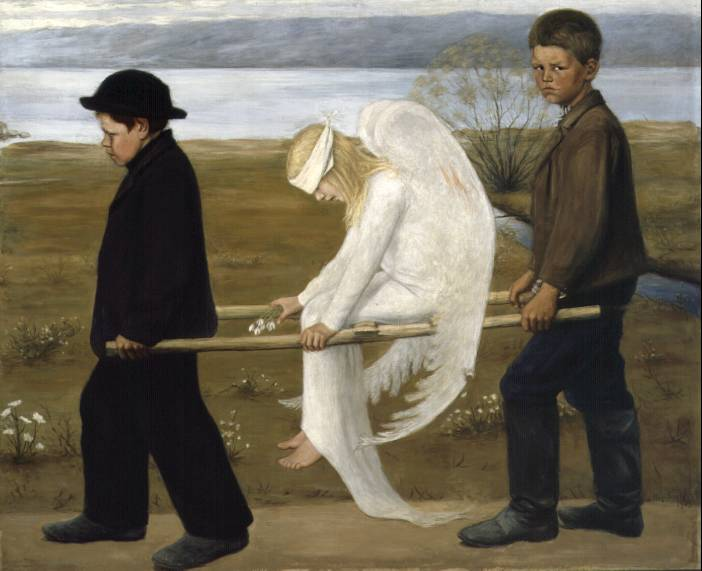
\includegraphics[scale=.20]{The_Wounded_Angel_-_Hugo_Simberg.jpg}\hfil
},{%
\hfil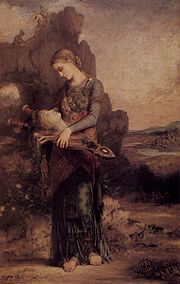
\includegraphics[scale=.4]{180px-Gustave_Moreau_007.jpg}\hfil
},{%
\hfil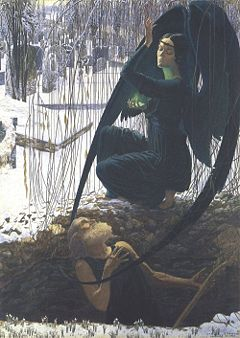
\includegraphics[scale=.4]{240px-Mort_du_fossoyeur.jpg}\hfil}}%
 \AQquestion[pq=1 cm]{Le tableau suivant a été peint par lequel de ces trois peintres ?\\
\hfil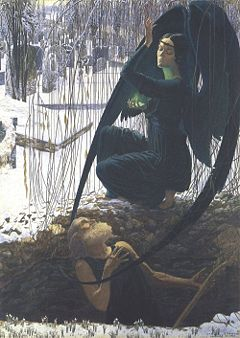
\includegraphics[height=3in]{240px-Mort_du_fossoyeur.jpg}\hfil}%
{{Gustav Klimt},{Carlos Schwabe},{Odilon Redon}}
\end{alterqcm} 

\begin{tkzltxexample}[small]
 \begin{alterqcm}[lq=8cm,numprop=true,sep]
 \AQquestion[pq=2 cm]{Parmi les trois tableaux, quel est celui peint par \textbf{Gustave Moreau}\vfill}%
 {{%
 \hfil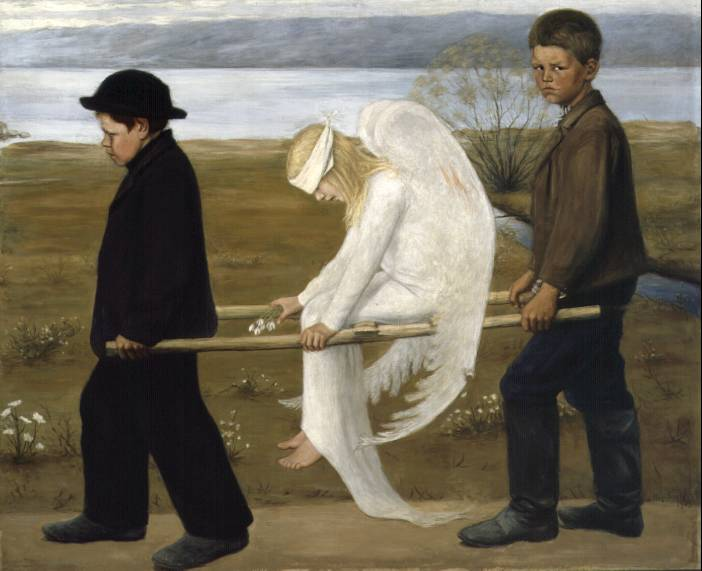
\includegraphics[scale=.25]{The_Wounded_Angel_-_Hugo_Simberg.jpg}\hfil
 },{%
 \hfil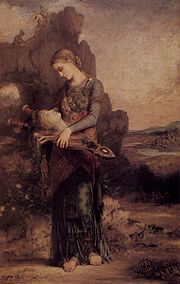
\includegraphics[scale=.5]{180px-Gustave_Moreau_007.jpg}\hfil
 },{%
 \hfil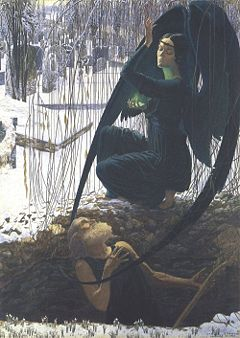
\includegraphics[scale=.4]{240px-Mort_du_fossoyeur.jpg}\hfil}}
  \AQquestion[pq=1 cm]{Le tableaux suivant, a été peint par lequel de ces trois peintres ?\\
 \hfil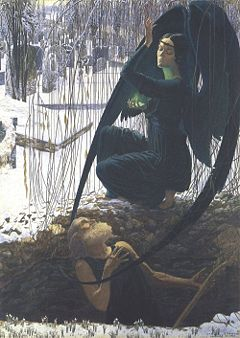
\includegraphics[height=3in]{240px-Mort_du_fossoyeur.jpg}\hfil}%
 {{Gustav Klimt},{Carlos Schwabe},{Odilon Redon}}
 \end{alterqcm} 
\end{tkzltxexample}

\subsection{Emploi d'un environnement \tkzname{tikzpicture} dans une question} 
\Ienv{tikzpicture}

\medskip

\begin{alterqcm}[lq=120mm,pre=true,pq=3mm]
 \AQmessage{\begin{minipage}{15cm}
\vspace*{6pt}   
Les trois arbres donnés ci-dessous représentent des situations probabilistes. %
  Les nombres indiqués sur les différentes flèches sont des  probabilités, et,%
    en deuxième niveau,  des probabilités conditionnelles. Ainsi pour l'arbre donné %
      dans la question 1 : $0,35 = P(A)$ et $0,1 =  P_{\text{A}}(E)$.
\vspace*{6pt}    
\end{minipage}  
}
\AQquestion{La probabilité de l'événement E est égale à : \\
\begin{tikzpicture}[yscale=1.2] 
[parent anchor=east,child anchor=west,grow=east]
\tikzstyle{every node}=[text=Maroon,fill=fondpaille,font=\small]
\tikzstyle{every child}=[level distance=25mm]
\tikzstyle{edge from parent}=[draw,->,thin] 
\tikzstyle{level 2}=[sibling distance=12mm]
\node {}
[grow=right]   
child {node {B}
      child { node {F}
        edge from parent node {$0,5$}}
      child { node {E}
        edge from parent node {$0,5$}
            }
         edge from parent node {$0,65$}
       }
child {node {A}
        child { node {F}
          edge from parentnode {$0,9$}}
        child { node {E}
          edge from parent node {$0,1$}}
      edge from parent node {$0,35$}
      };
\end{tikzpicture}}
{{$0,5$},%
{$0,1$},%
{$0,6$},%
{$0,36$}}
\end{alterqcm} 

\begin{tkzltxexample}[small]
 \begin{alterqcm}[lq=120mm,pre=true,pq=3mm]
  \AQmessage{Les trois arbres donnés ci-dessous représentent des situations probabilistes.
   Les nombres indiqués sur les différentes flèches sont des  probabilités, et,
   en deuxième niveau,  des probabilités conditionnelles. Ainsi pour l'arbre donné 
   dans la question 1 : $0,35 = P(A)$ et $0,1 =  P_{\text{A}}(E)$.}
 \AQquestion{La probabilité de l'événement E est égale à : \\
 \begin{tikzpicture} 
 ...
 \end{tikzpicture}}
 {{$0,5$},%
 {$0,1$},%
 {$0,6$},%
 {$0,36$}}
 \end{alterqcm} 
\end{tkzltxexample}

\subsection{Emploi d'un environnement \tkzname{array} dans les propositions} 
\Ienv{array}

Il est possible d'utiliser des tableaux ainsi que d'autres structures dans le code de la question ou encore des propositions. Voici un exemple :

\medskip


\begin{tkzexample}[vbox]
\begin{alterqcm}[lq=88mm,symb=$\Box$]
\AQquestion{Le couple $(1~;~-1)$ est solution de }
{%
{$ \left\lbrace
\begin{array}{ll}
 0,75a + 0,5b &= 0,25 \\
 0,25a + 0,5b &=-0,25
\end{array}\right.$},
{$ \left\{
\begin{array}{ll}
 a &=  0,75a +0,5b \\
 b &=  0,25a +0,5b
\end{array}\right.$},
{$ \left\lbrace
\begin{array}{ll}
 0,75a - 0,5b &= 0,25 \\
 0,5a + 0,25b &=-0,25
\end{array}\right.$}
}
\end{alterqcm}\end{tkzexample}  

\subsection{Emploi d'un environnement \tkzname{tikzpicture} dans une question} 
\Ienv{tikzpicture}

\begin{tkzexample}[vbox]
\begin{alterqcm}[lq=8cm,numprop=true,sep]
\AQquestion{Parmi les figures ci-contre, indiquer celle qui est un losange :}
{{\hspace{1cm}  \begin{minipage}{5cm} \begin{tikzpicture} 
  \draw (0,0)--(1.5,0)--(2,1)--(.5,1)--cycle; 
\end{tikzpicture} \end{minipage}},
{\hspace{1cm}  \begin{minipage}{5cm} \begin{tikzpicture}
   \draw[rotate=30] (0,0) rectangle (1.5,1); \end{tikzpicture} \end{minipage}},
{\hspace{1cm}  \begin{minipage}{5cm} \begin{tikzpicture}
   \draw (0,0) rectangle (1,1); \end{tikzpicture} \end{minipage} }}
\end{alterqcm} 
\end{tkzexample}

\subsection{Emploi de code \tkzname{verbatim} dans les questions et les propositions} 
\Ienv{verbatim}

Voici un exemple de Pascal Bertolino. Il est préférable d'utiliser comme Pascal l'a fait la macro \tkzcname{texttt}, autrement d'éviter l'usage du mode 
|verbatim|. Nous verrons à la page suivante comment procéder si ce mode est réellement nécessaire.

\begin{alterqcm}[lq=80mm,title=false,long] 

%--------------------------------------------------------------
\AQquestion{Quel était le langage précurseur du langage C ?}
{{le Fortran},
 {le langage B},
 {le Basic}}

%--------------------------------------------------------------
\verbdef\argprop|int a = 3 ^ 4 ;|
\AQquestion{\argprop}
{{élève 3 à la puissance 4},
 {fait un OU exclusif entre 3 et 4},
 {n'est pas une instruction C}}

%--------------------------------------------------------------
\AQquestion{Quelle est la bonne syntaxe pour décaler de 8 bits à gauche l'entier \texttt{a} ?}
{{\texttt{b = lshift(a, 8) ;}},
 {\texttt{b = 8 << a ;}},
 {\texttt{b = a << 8 ;}}}
%--------------------------------------------------------------
\verbdef\argprop|{ printf ("bonjour") ; return 0 ; \}|
\AQquestion{Le programme complet :	\\
\texttt{int main() \\
~~\argprop}}
{{affiche \texttt{bonjour}},
 {donne une erreur à la compilation},
 {donne une erreur à l'exécution}}
%--------------------------------------------------------------
\verbdef\arg|float tab[10]|
\verbdef\propa|*tab|\global\let\propa\propa
\verbdef\propb|&tab|\global\let\propb\propb
\verbdef\propc|tab|\global\let\propc\propc
\AQquestion{Soit la déclaration \arg ; \\Le premier réel du tableau  est \ldots}
{{\propa},
 {\propb},
 {\propc}}

%--------------------------------------------------------------
\AQquestion{La ligne \texttt{printf("\%c", argv[2][0]) ;} du \texttt{main} de  \texttt{monProg} exécuté ainsi : 
\texttt{monProg parametre }}
{{affiche \texttt{p}},
 {n'affiche rien},
 {peut provoquer un plantage}}
%--------------------------------------------------------------
\AQquestion{Quelle est la taille en mémoire d'un \texttt{long int} ?}
{{4 octets},
 {8 octets},
 {ça dépend \ldots}}
%--------------------------------------------------------------
\AQquestion{Suite à la déclaration \texttt{int * i} ;}
{{\texttt{*i} est une adresse},
 {\texttt{*i} est un entier},
 {\texttt{*i} est un pointeur}}
%--------------------------------------------------------------
\AQquestion{Un des choix suivants n'est pas une bibliothèque standard du C}
{{\texttt{stdlib}},
 {\texttt{stdin}},
 {\texttt{math}}}

\end{alterqcm}

\medskip
Voyons le code source

le plus simple est souvent d'utiliser la commande \tkzcname{texttt}

\medskip
\begin{tkzexample}[code only]
 \AQquestion{Suite à la déclaration \texttt{int * i} ;}
 {{\texttt{*i} est une adresse},
 {\texttt{*i} est un entier},
 {\texttt{*i} est un pointeur}}
\end{tkzexample}

\medskip
\begin{tkzexample}[code only]
\AQquestion{La ligne \texttt{printf("\%c", argv[2][0]) ;}
 du \texttt{main} de  \texttt{monProg} exécuté ainsi : 
\texttt{monProg parametre }}
{{affiche \texttt{p}},
 {n'affiche rien},
 {peut provoquer un plantage}}
\end{tkzexample}

\medskip
Sinon on peut charger le package \tkzname{verbdef} :
\NamePack{verbdef}

\medskip
\tkzcname{usepackage\{verbdef\}}

\medskip
\begin{tkzexample}[code only]
 \verbdef\argprop|int a = 3 ^ 4 ;|
 \AQquestion{\argprop}
 {{élève 3 à la puissance 4},
  {fait un OU exclusif entre 3 et 4},
  {n'est pas une instruction C}}
\end{tkzexample}

\medskip
Il est possible que plusieurs variables soient nécessaires :

\medskip

\begin{tkzexample}[code only]
 \verbdef\arg|float tab[10]|
 \verbdef\propa|*tab|\global\let\propa\propa
 \verbdef\propb|&tab|\global\let\propb\propb
 \verbdef\propc|tab|\global\let\propc\propc
 \AQquestion{Soit la déclaration \arg ; \\
 Le premier réel du tableau  est \ldots}
 {{\propa},
  {\propb},
  {\propc}}
\end{tkzexample}



\endinput
\section{Points attibués à un QCM}

Il est possible d'attribuer des points à un QCM à l'aide de la macro rudimentaire suivante \tkzcname{AQpoints}

\begin{tkzltxexample}[small]
 \newcommand\AQpoints[1]{%
 \marginpar{\hspace*{1em}    
 \begin{tabular}{|c|}
   \hline  
   \textbf{#1}\\ 
   \hline\\ 
   \hline 
 \end{tabular}}} 
\end{tkzltxexample}
  
\subsection{Exemple} 

\begin{tkzltxexample}[]
    \AQpoints{10}
  \begin{alterqcm}[symb = \dingsquare, lq=7cm]
  \AQquestion{Si \numprint{3,24} est la troncature de $x$ au centième, alors on est sûr que :}
  {{\begin{minipage}[t]{\linewidth-1cm}$3,235\leqslant x <3,245$\\
    \end{minipage}} ,
   {\begin{minipage}[t]{\linewidth-1cm} $3,24\leqslant x <3,25$\\
    \end{minipage}} ,
   {\begin{minipage}[t]{\linewidth-1cm}
       $x$ est plus près de \numprint{3,24} que de \numprint{3,25}
    \end{minipage}}}
  \end{alterqcm}
\end{tkzltxexample}

\medskip
\AQpoints{10}
  \begin{alterqcm}[symb = \dingsquare, lq=7cm]
  \AQquestion{Si \numprint{3,24} est la troncature de $x$ au centième, alors on est sûr que :}
  {{\begin{minipage}[t]{\linewidth-1cm}$3,235\leqslant x <3,245$\\
    \end{minipage}} ,
   {\begin{minipage}[t]{\linewidth-1cm} $3,24\leqslant x <3,25$\\
    \end{minipage}} ,
   {\begin{minipage}[t]{\linewidth-1cm}
       $x$ est plus près de \numprint{3,24} que de \numprint{3,25}
    \end{minipage}}}
\end{alterqcm}   
\endinput  
\section{Problèmes connus et FAQ}

\subsection{Incompatibilité avec \tkzname{colortbl.sty}}

 Le problème provient du fait que \tkzname{colortbl.sty} est parfois incompatible avec la commande \tkzname{multicolumn}. Le texte utilisé dans la commande \tkzname{multicolumn} ne doit contenir qu'un seul paragraphe. 
 Il faut simplement ne pas utiliser la commande \tkzname{AQmessage}. Une solution est d'interrompre le QCM pour afficher ce que l'on souhaite puis reprendre le tableau.
 
 \subsection{FAQ}
  \subsubsection{Traduction des commandes}
  Certaines commandes peuvent être traduites ou modifiées comme par exemple : \tkzcname{aq@pre}  et \tkzcname{aq@preVF}, il suffit pour cela d'utiliser \tkzcname{renewcommand} 
  
\begin{tkzltxexample}[]
 \renewcommand{\aq@pre}{Pour chacune des questions ci-dessous, une seule des
  r\'eponses propos\'ees est exacte. Vous devez  cocher la r\'eponse exacte
   sans justification.
 Une bonne r\'eponse rapporte \textbf{\cmdAQ@global@bonus\ point}. Une
  mauvaise r\'eponse enl\`eve \textbf{\cmdAQ@global@malus\ point}.  L'absence
  de r\'eponse ne rapporte ni n'enl\`eve aucun point. Si le total des points
  est n\'egatif, la note globale attribu\'ee \`a l'exercice est \textbf{0}.}% 
\end{tkzltxexample}

  
\endinput  

\clearpage\newpage 
\makeatletter    
\printindex  
\end{document}

